\section{Evaluation}~\label{sec:exp}
We first applied our approaches to several real-world dataset and compare our method with the uniform random sampling. Then we conduct several user studies on specific analysis tasks. 
\subsection{Case Study}
In this section, we evaluate our method by presenting the applications on two taxi trajectory datasets: Porto and Shenzhen. We compare the visualization among the full dataset, random sampling and the proposed method from multiple levels of details. 
\subsubsection{Case of Porto Distinct}
Our first example uses taxi trajectories collected from 442 active taxis in Porto distinct, Portugal~\footnote{\url{http://www.geolink.pt/ecmlpkdd2015-challenge/dataset.html}}. The trajectories cover several cities in and around the Porto distinct and has been cleaned for further analysis.


\stitle{Overview of the Porto Distinct}
Figure~\ref{fig:teaser} C presents the visualization generated by the whole dataset, from which we can get an overview of the movement patterns in Porto district. For example, large number of trajectories are concentrated in the center of the figure(shown around Figure~\ref{fig:teaser} C$_1$) indicating that the most taxi activities are around the \UC{Porto City}. In addition, 
many trajectory clusters distributed across the land indicate the locations of other cities in Porto district(shown as the dash circle in Figure~\ref{fig:teaser} C). 

We compare the $\avats$ with \textit{uniform random sampling} at the overview. 
Figure~\ref{fig:teaser} B and E show the visualization generated by uniform random sampling and $\avats$ respectively. Both of these two sampling methods take 0.01 as the sampling rate. The uniform random sampling almost only preserves the visual structure around the Porto City and the trajectories at the marginal regions are lost.
The visualization generated by $\avats$ looks close to the whole dataset. Not only the \UC{Porto City} but also the margin city structure are well preserved, which are shown as the dash circles in ~\ref{fig:teaser} E.
 
Furthermore, the color encoding further enhances the visualization by revealing the \QM{representativeness} of the trajectories.
As shown by Figure~\ref{fig:teaser} E$_1$, there is no clear pattern can be discovered due to the dense concentration of massive trajectories. While in Figure~\ref{fig:teaser} F$_1$, some trajectories with high representative score are highlighted by dark orange color such as F$_2$, which indicates Avenida da Boavista, a main avenue in Porto City. 
%From the overview, $\avats$ can preserve the general structure very well in the comparison with uniform random sampling, and more information of the movement can be visualized with color encoding.
 
 
An important factor affecting the visual fidelity of sampling results is the sampling rate. Figure~\ref{fig:teaser} B and C show the sampling results of random method with sampling rate set as 0.01 and 0.001. With the decreasing of the sampling rate, the shape of the trajectory visualizations clearly shrink to the Porto City and result to the loss of visual fidelity at the marginal region. Figure\ref{fig:teaser} E and D demonstrate the visualization of $\avats$ with the sampling rate of 0.01 and 0.001. We observe that when the sampling rate is decreased, the framework of the trajectories remains the same but the trajectories around Porto City are significantly removed because more \QM{blank space/gap} can be found in the center of figure as shown in Figure~\ref{fig:teaser} D$_1$. 

\stitle{Detail view of Porto Distinct}
To demonstrate the effectiveness of $\avats$ at detail view, we select three regions of interest(as shown in the Figure\ref{fig:porto} A), which have different trajectory density and generate the visualization by setting the map level of 14) 
   
Region R3 is far away from Porto City and contains two other cities: Paredes and Penafiel. Region R3 has very few trajectories as shown in Figure~\ref{fig:porto} D$_1$.  Compare with the visualization of full dataset, the random sampling almost misses all trajectories in this region(as shown in Figure~\ref{fig:porto} D$_2$). While $\vats$ samples much more trajectories than random sampling as shown in Figure~\ref{fig:porto} D$_3$. However, some meaningful structure are still missing such as the trajectory bundle shown in Figure~\ref{fig:porto} h, which is laid in on the road \QM{road name} connecting the two cities of Paredes and Penafiel. Further more, the trajectory structure of city Penafiel is not precisely preserved(shown as region g in Figure~\ref{fig:porto} D$_3$ i) because some  trajectory branches are missed.  
By setting the representative parameter as 64, $\avats$ generate a more confidential visualization than $\vats$ shown as Figure~\ref{fig:porto} D$_4$. 

Region 2 is near to the center of Porto have are more taxi trajectories. There are three cities located in the region R2 including Ermesinde, Rio Tinto and Valongo.  
Figure~\ref{fig:porto} C$_2$ and C$_3$ present the visualization generated by $\avats$ with the representative parameters of 4 and 64. We observe that the visualization shown in Figure~\ref{fig:porto} C$_3$ have more details trajectory branches than Figure~\ref{fig:porto} C$_3$(as shown in regions c,d of Figure~\ref{fig:porto} C$_2$ and C$_3$). In this case, a larger representative parameter is more beneficial in preserving the details at this level. Furthermore, Figure~\ref{fig:porto} C$_4$ shows the visualization of $\avats$($delta = 64$) with color encoding. In the comparison with Figure~\ref{fig:porto} C$_3$, the visualization in Figure~\ref{fig:porto} further highlights the movement distribution. 
For instance, we observe that region $f$ in Figure~\ref{fig:porto} C$_4$ has more deep colored trajectories than region $e$ and $g$, thus we inspect that city of Rio Tinto has more taxi trajectories than other two cities.
%For instance, we inspect that city Rio Tinto has more taxi trajectories than other two cities because.

The region R1 is the center of Porto city, which has the highest concentration of the trajectories and cause serious visual clutter if all trajectories are visualized(as shown in Figure\ref{fig:porto} B$_1$). $\avats$($delta = 4$) greatly alleviates the visual clutter and preserves the framework which basically follows the road network as shown in Figure~\ref{fig:porto} B$_2$. Furthermore, when setting the representative parameter $delta$ as 64, the structure is more clear as shown in region b of Figure~\ref{fig:porto} B$_3$ and B$_4$, and have more trajectory details than $\avats$($delta = 4$) as shown in region $a$ of Figure~\ref{fig:porto} B$_2$ and B$_3$. The trajectories with color encoding further enhance the visualization thus the audiences can compare the traffic flow of two route more easily.   
 
 

\begin{figure*}[t]
	\centering
	\vspace{2mm}
	\includegraphics[width=0.98\textwidth]{pictures/experiment_study/case_porto.pdf}
	\caption{Visualization at dense and sparse region respectively.}
	\vspace{0mm}
	\label{fig:porto}
\end{figure*}

\begin{figure}[t]
	\centering
	\vspace{2mm}
	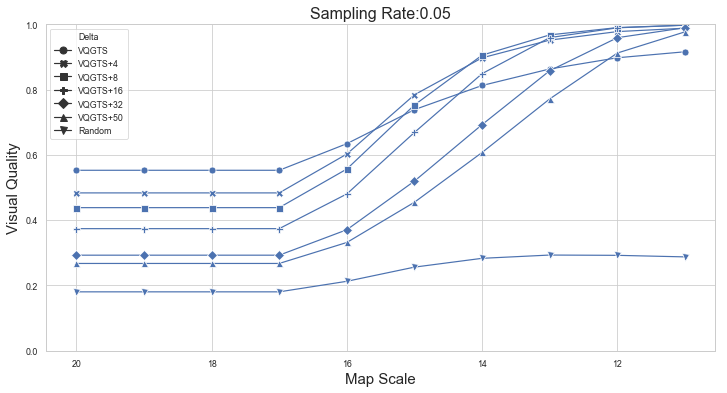
\includegraphics[width=0.45\textwidth]{pictures/experiment_study/quanlity.png}
	\caption{Visual quality chart. X axis indicates map scale from detail view to overview; y axis indicate the visual quality. }
	\vspace{0mm}
	\label{fig:quality_chart}
\end{figure}


\subsubsection{Shenzhen Trajectories}
We further evaluate the proposed approach using the taxi trajectories of Shenzhen, a booming city in the southern China and has very different urban form from Porto District. The dataset we used includes 428K taxi trajectories collected from \QM{**} taxis in one day. All the visualization generated by the sampling methods which sets the sampling rates as 0.01.
 
\stitle{Overview of Shenzhen}
Figure~\ref{fig:shenzhen} A-D present the overview visualization generated by whole dateset, random sampling, $\avats$ and $\avats$ with color encoding at the top level. The visualization of raw dataset(Figure~\ref{fig:shenzhen} A) shows the there are several dense trajectory clusters in southern districts of Shenzhen, including \textit{Baoan}, \textit{Nanshan}, \textit{Futian} and \textit{Luohu} districts, which are the most prosperous commercial zones of Shenzhen. Figure~\ref{fig:shenzhen} B presents the trajectories generated by random sampling. We observe that the most of the trajectories sampled by random sampling are located at the commercial zones. On the other hand, the trajectories at the north Shenzhen are missing, thus making the visualization visually different from the whole dataset.
$\avats$ outperforms random method by guaranteeing the spatial coverage of the whole trajectories thus result in a higher visual fidelity. Further more, some isolate trajectories are still preserved shown in Figure~\ref{fig:shenzhen} C. $\avats$ with color is able to reveal the spatial distribution of the trajectories. For example, for the regions a, b in Figure~\ref{fig:shenzhen} A or C, the visualization is unable to explain which region has more taxi activities because both of these two regions are fully covered by trajectories. In Figure~\ref{fig:shenzhen} D, we find the more trajectories encoded by deep color are found in region a than that of region b, which indicates more trajectories can be found in region a than region b. 

\stitle{Detail view of Shenzhen}
Then we narrow down to the region of airport. Compare with visualization of whole dataset(shown as Figure~\ref{fig:shenzhen} E), the random sampling only preserves the trajectories pass through several routes with very high traffic flow(shown as Figure~\ref{fig:shenzhen} F).  Both $\avats$ and $\avats$ with color encoding can visualize the trajectory structure very well. The $\avats$ with color encoding further enriches the information by encoding the trajectory with color. For example, we can observe that there are more trajectories pass through G4 and G104 than Baoan Avenue, which is hard to be discovered from the Figure~\ref{fig:shenzhen} E, F and G.  

Similarly, in the region near to the Shenzhen North Railway Station, the visualization generated by $\avats$ can reveal some road structure such as the \QM{round entrance to the motorway} shown as region c in Figure~\ref{fig:shenzhen} K. With the color encoding, we can also easily discover that the road G94 have a higher road traffic flow than the Minzhi avenue and Mellon avenue as shown in Figure~\ref{fig:shenzhen} L.

\begin{figure*}[t]
	\centering
	\vspace{2mm}
	\includegraphics[width=0.98\textwidth]{pictures/experiment_study/case_shenzhen.pdf}
	\caption{Case study of Shenzhen.}
	\vspace{0mm}
	\label{fig:shenzhen}
\end{figure*}


\subsection{User Study}
To further evaluate the effectiveness of $\avats$ from the the audience perspective, we conducted formal user studies to compare how users perform the urban exploration tasks with visualizations generated by whole dataset, \textit{random sampling} and $\avats$.


\begin{figure}[t]
	\centering
	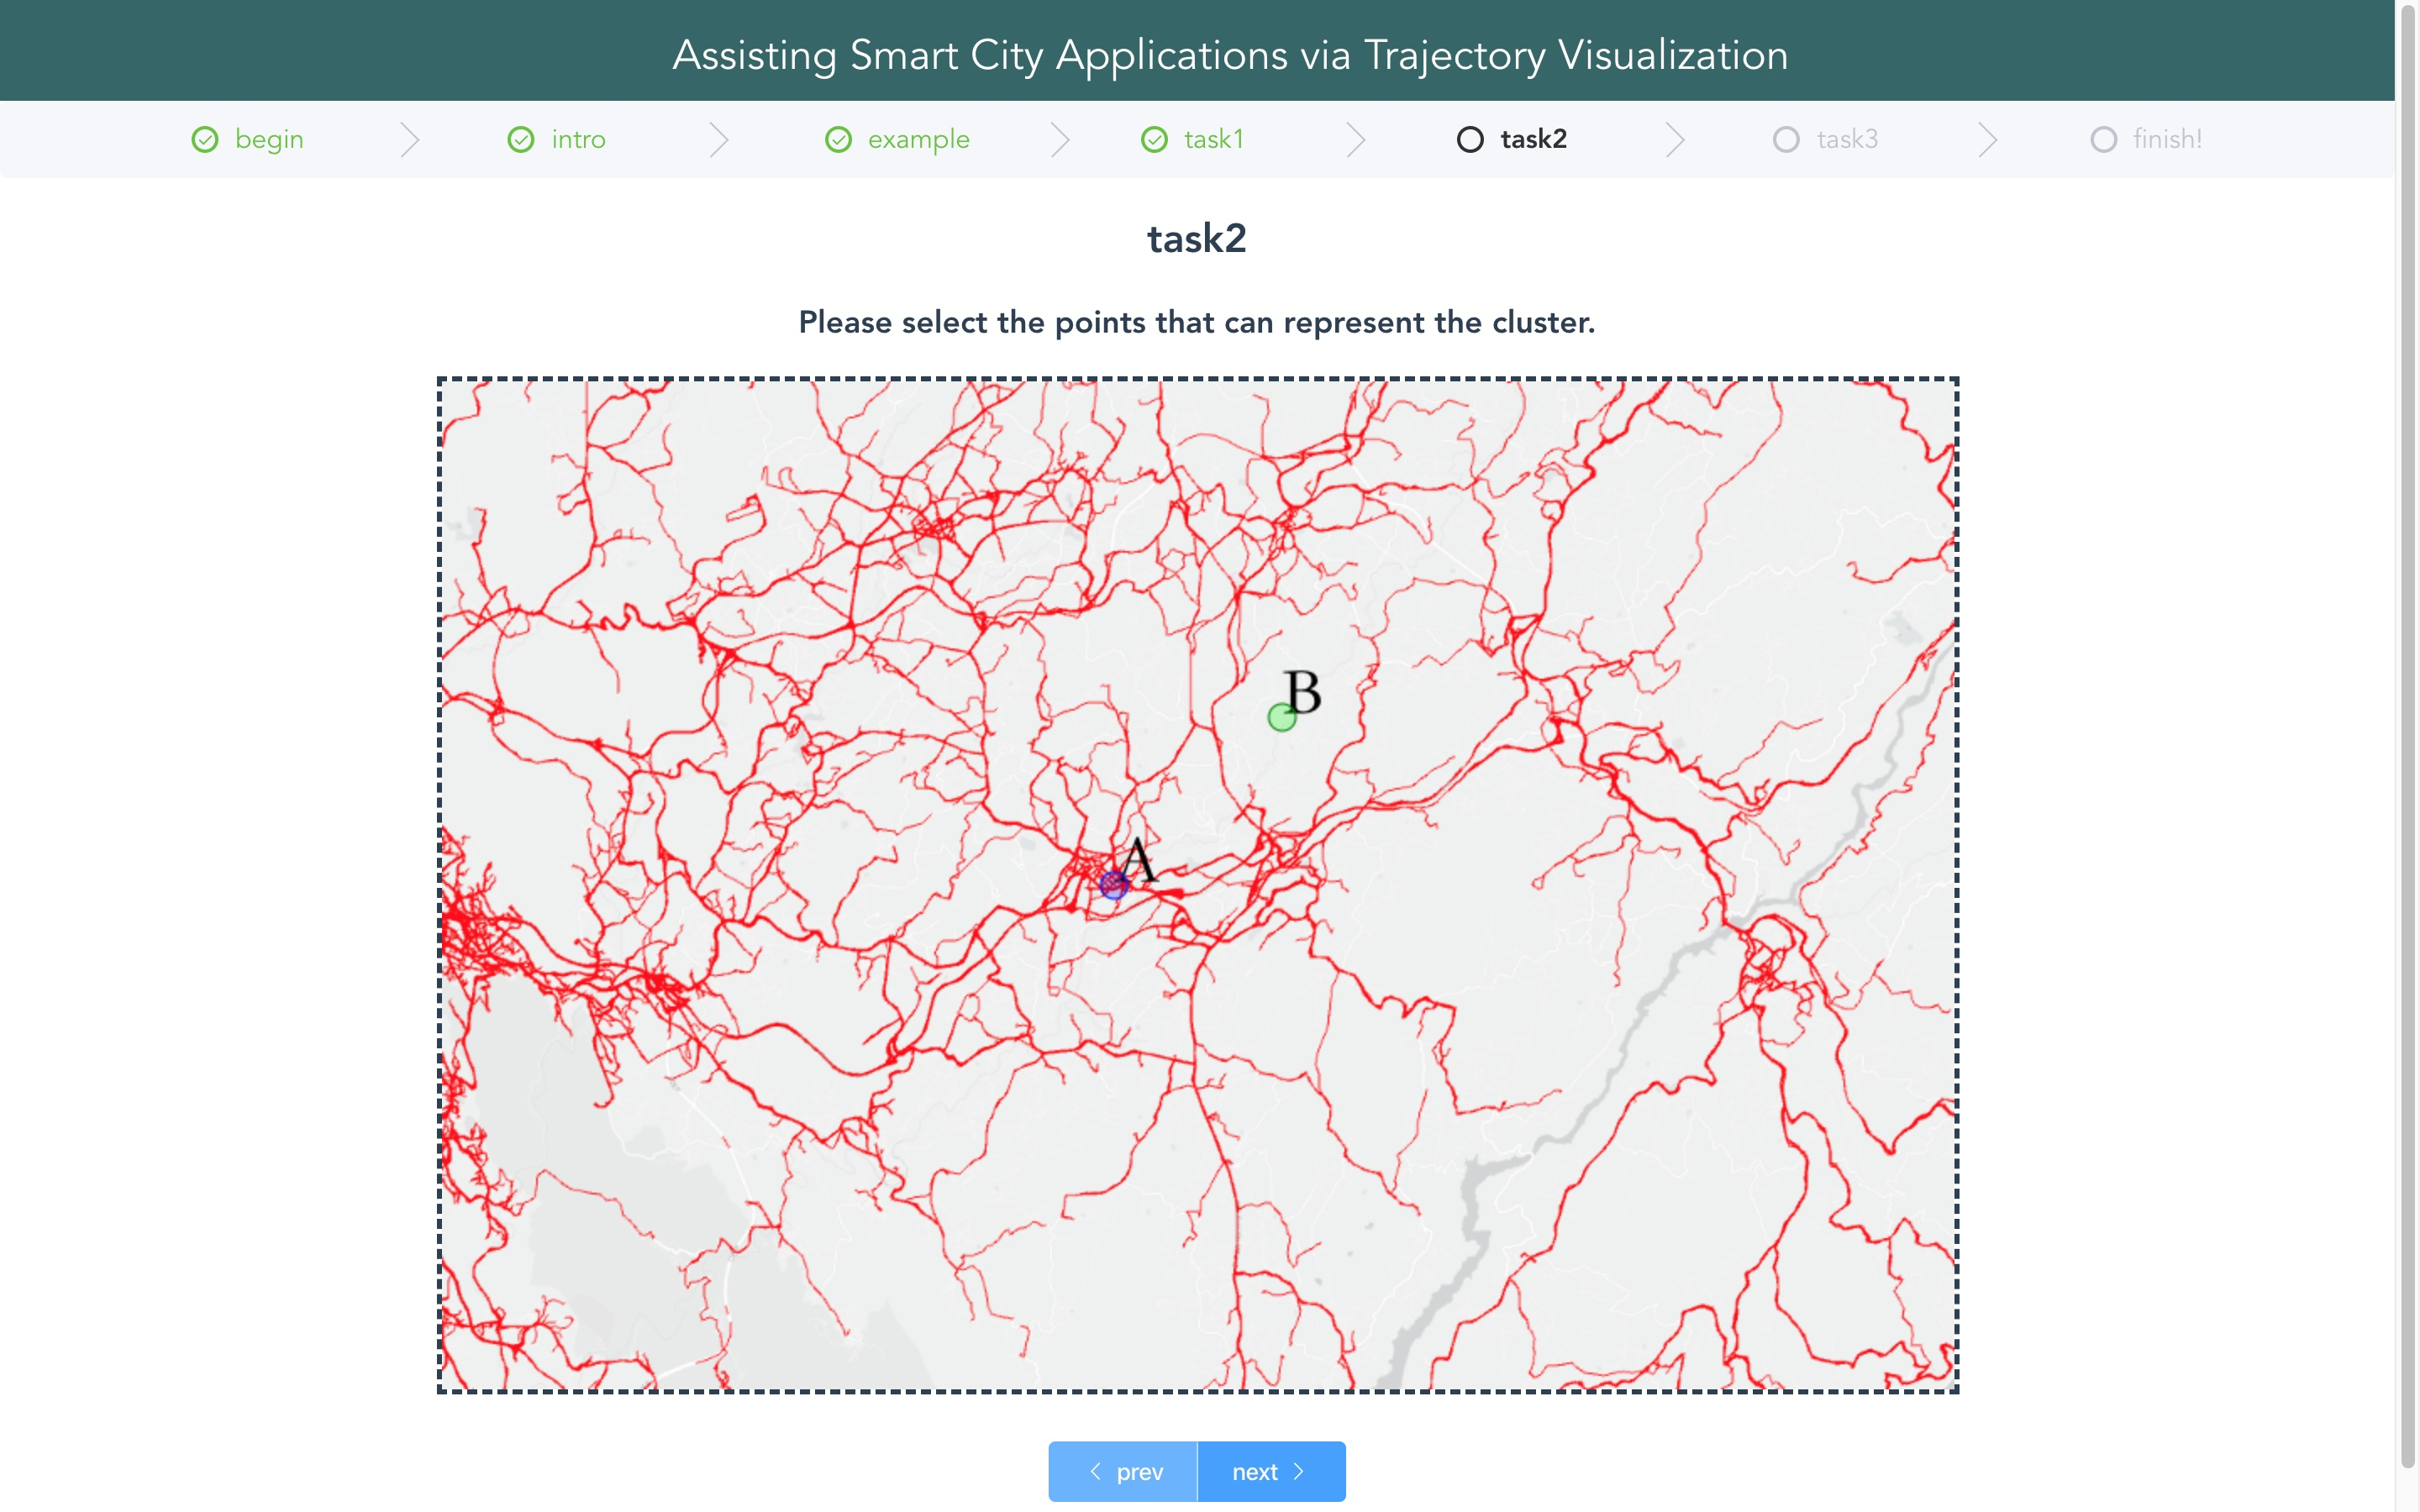
\includegraphics[width=0.44\textwidth]{pictures/user_study/interface.jpg}
	\vspace{-3mm}
	\caption{The interface of user study platform.}
	\vspace{-5mm}
	\label{fig:user_study}
\end{figure}

\subsubsection{Experiment setting}

\stitle{Participants and apparatus}
We recruit 100 participants (** females, ** males, aged 20 to **(mean=**, SD=**)) with normal vision or normal corrected vision. All of these participants have the background of computer science. 
The study system is a web-based platform which has the fixed size of interface and the participants perform the user study on their own  computers.  The system interface is shown as Figure~\ref{fig:user_study}. Considering the unfairness caused by the screen size, we recommend all participants to set the resolution of the screen as 1980 * 1080 before the experiment. All images displayed on the interface have the same size of(AA*BB).  

\stitle{Tasks and data generation.}
All participants needed to perform four types of tasks:
\setlist{nolistsep}
\begin{itemize}[noitemsep]
	\item \textbf{T1. Traffic flow estimation.} 
	The participants are asked to select the route with higher traffic flow from two candidate road segments
	\item \textbf{T2. \QM{Trajectory cluster} identification.} The participants need to identify the centers of the cities or commercial regions from the trajectory visualization.
	\item \textbf{T3. Route inspection.} The participants were asked to inspect the reachable routes between the two regions by draw lines or push the button indicating uncertain.
	\item \textbf{T4. Visual similarity comparison.} With a given visualization generated by full dataset as ground truth, the participants were asked to rank a set of visualizations according to the similarity to the ground truth. 
\end{itemize}

\stitle{Data generation}
We used the taxi trajectory dataset of Porto and Shenzhen for the user study. The testing data for each type of tasks were generate as follows:

\textbf{Tasks of T1.} We selected several visualization views which contain enough clear road structure. Then the number of trajectories passing through each road segment were counted as the traffic flow of this road segment. In the tasks of T1, two road segments are given randomly, and the users needed to select the one with higher traffic flow.  

\textbf{Tasks of T2.} We randomly chose several visualization views which contain city/commercial regions and labeled the locations of each city/commercial region centers on the visualization as the correct locations first.  Then we randomly generated locations and remove the locations close to the correct locations, the remaining locations are the error locations. In each task of T2, with a given visualization, the same number of correct and wrong locations will be randomly selected and the participants were asked to select the locations indicating the city/commercial regions centers. 

\textbf{Tasks of T3.} We randomly chose several visualization views which contain two or more city/commercial regions. In the tasks of T3, the users were asked to draw the reachable routes between the two selected regions. 

\textbf{Tasks of T4.} With a given center location and zoom scale, we generated the visualizations by using whole dataset, uniform random sampling and $\avats$ with different parameters. Using visualization generated by whole dataset as ground truth, users were required to score the other visualizations according to the similarity to the ground truth.  

\stitle{Procedure}
The user study began with the introduction, in which the motivation, tasks and visual encoding were introduced. The following sessions are divided into four blocks according to the task types. Each block starts with a task tutorial, in which the participants could perform several demo tasks and were free to ask questions, thus familiarizing themselves with the interface, interaction and tasks.
Then the users were asked to finish five normal tasks. During this procedure, both the answer and the time usage are recorded.
After all tasks were finished, the participants would fill a questionnaire about their comments. 

\subsubsection{Results}

\stitle{Accuracy}

\stitle{Time usage}

\stitle{User feedback}